
\chapter{Initialization}\index{initialization (of you)}
\label{ch:introduction}

\epigraph{The simulation is such that [one] generally perceives the sum of many billions of elementary processes simultaneously, so that the leveling law of large numbers completely obscures the real nature of the individual processes.}{John von Neumann\index{von Neumann, John} \cite{von2018mathematical}}











\noindent{}Thanks to substantial investments into computer technology, modern \term{artificial intelligence} (AI) systems can now come equipped with many billions of elementary components. When these components are properly 
initialized 
and then trained, AI can accomplish tasks once considered so incredibly complex that philosophers have previously argued that only \emph{natural} intelligence systems -- i.e.~humans -- could perform them. 


Behind much of this success in AI is \term{deep learning}. Deep learning uses artificial \textbf{neural networks}\index{neural network|textbf} as an underlying model for AI: while loosely based on \emph{biological} neural networks\index{biological neural network|seealso{brain}}\index{biological neural network} such as your \terminate{brain}, \emph{artificial} neural networks are probably best thought of as an especially nice way of specifying a flexible set of functions, built out of many basic computational blocks called \textbf{neurons}\index{neuron|textbf}. This model of computation is actually quite different from the one used to power the computer you're likely using to read this book. In particular, rather than \emph{programming} a specific set of instructions to solve a problem directly, deep learning models  are \emph{trained}
on data from the real world and learn how to solve problems.




The real power of the deep learning framework comes from \emph{deep} neural networks, with many neurons in parallel organized into sequential computational layers,  \emph{learning} useful representations of the world. 
Such \term{representation learning} transforms data into increasingly refined forms that are helpful for solving an underlying task, and is thought to be a hallmark of success in intelligence, both artificial and biological.













Despite these successes and the intense interest they created, deep learning \emph{theory} is still in its infancy. 
Indeed, there is a serious disconnect between theory and practice: while practitioners have reached amazing milestones, they have far outpaced the theorists,
whose analyses often involve assumptions
so unrealistic that they lead to conclusions that are irrelevant to understanding deep neural networks as they are typically used. 
More importantly,
very little theoretical work directly confronts
the \emph{deep} of deep learning, despite a mass of empirical evidence for its importance in the success of the framework.





\index{principle!InfoMax|see{InfoMax principle}}
\index{principle!of indifference|see{Laplace's principle of indifference}}
\index{principle!maximum entropy|see{maximum entropy, principle}}
\index{principle!learning-rate equivalence|see{equivalence principle}}
\index{principle!criticality|see{criticality}}
\index{principle!sparsity and near-sparsity|see{sparsity, principle of}}
\index{principle!typicality|see{typicality}}
\index{principle!variational|see{variational principle}}

The goal of this book is to put forth
a set of \textbf{principles}\index{principle|textbf} that enable us to theoretically analyze \emph{deep} neural networks of \emph{actual relevance}.  
To initialize you to this task, in the rest of this chapter
we'll explain at a very high-level both \emph{(i)} why such a goal is even attainable in theory 
and \emph{(ii)} how we are able to get there in practice.











\section{An Effective Theory Approach}\label{sec:ET-approach}
\epigraph{Steam navigation brings nearer together the most distant nations. \ldots their theory is very little understood, and the attempts to improve them are still directed almost by chance. \ldots We propose now to submit these questions to a deliberate examination.}{Sadi Carnot, commenting on the need for a theory of deep learning \cite{carnot1890reflections}.\index{Carnot, Sadi}}



\index{microscopic perspective}\index{microscopic perspective|seealso{parameter space}}
\noindent{}While modern deep learning models are built up from seemingly innumerable elementary computational components, a first-principles \emph{microscopic} description of \emph{how} a trained neural network computes a function from these low-level components is entirely manifest.
This microscopic description is just the set of instructions for transforming an input through the many layers of  components into an output. Importantly, during the training process, these components become very finely-tuned, and knowledge of the particular tunings is necessary for a system to produce useful output.

\index{macroscopic perspective}\index{macroscopic perspective|seealso{sample space}}
Unfortunately, the complexity of these tunings obscures any first-principles \emph{macroscopic} understanding of \emph{why} a deep neural network computes a particular function and not another.
With many
neurons performing different tasks as part of such a computation, it seems hopeless 
to think that we can use theory to understand these models at all, and 
silly to believe that
a small set of 
mathematical \emph{principles}
will be sufficient for that job.

Fortunately, \textbf{theoretical physics}\index{physics|textbf} has a long tradition of finding simple \textbf{effective theories}\index{effective theory|textbf} 
of complicated systems with a large number of components. 
The immense success of the program of physics in modeling our physical universe 
suggests that perhaps some of the same tools may be useful for theoretically understanding deep neural networks.
To motivate this connection, let's very briefly reflect on the successes of thermodynamics and statistical mechanics, physical theories that
together explain from microscopic first principles the macroscopic behavior of systems with many elementary constituents.













A scientific consequence of the 
\terminate{Industrial Age}, %
\textbf{thermodynamics}\index{thermodynamics} arose out of an effort to describe and innovate upon the \terminate{steam engine} -- a system consisting of many many particles and perhaps the original \neo{black box}. The laws of thermodynamics, derived from careful empirical observations, were used to codify the mechanics of steam, providing a high-level understanding of these macroscopic \emph{artificial} machines that were transforming society. While the advent of thermodynamics led to tremendous improvements in the efficiency of steam power, its laws were in no way
fundamental.

It wasn't until much later that Maxwell\index{Maxwell, James Clerk}, Boltzmann\index{Boltzmann, Ludwig}, and Gibbs\index{Gibbs, J. Willard} provided the missing link between experimentally-derived effective description on the one hand and a first-principles theory on the other hand.
Their \textbf{statistical mechanics}\index{statistical physics|textbf}\index{statistical mechanics|see{statistical physics}} explains how the macroscopic laws of thermodynamics describing human-scale machines could arise \emph{statistically} from the deterministic dynamics of many microscopic elementary constituents. 
From this perspective, the laws of thermodynamics were \emph{emergent} phenomena that only appear from the collective statistical behavior of a very large number of microscopic particles.
In fact, it was the detailed theoretical predictions derived from statistical mechanics that ultimately led to the general scientific acceptance 
that \terminate{matter} is really comprised of molecules\index{molecule} and atoms\index{atom}.
Relentless application of statistical mechanics
led to the discovery of \neo{quantum mechanics}, which 
is a precursor to the
invention of the \terminate{transistor} that powers the \terminate{Information Age}, and 
-- taking the long view -- 
is what has allowed us to 
begin to 
realize artificial machines that can 
think %
intelligently.








Notably, these physical theories originated from a desire to understand \emph{artificial} human-engineered objects, such as the steam engine. Despite a 
potential %
misconception, \terminate{physics}  doesn't make a distinction between natural and artificial phenomena. Most fundamentally, it's concerned with providing a unified set of principles that account for past empirical observations and predict the result of future experiments; the point of theoretical calculations is to connect measurable outcomes or \textbf{observables}\index{observable|textbf} directly to the fundamental underlying constants or \textbf{parameters}\index{model parameters!connection to observables} that define the theory. This perspective also implies a tradeoff between the predictive 
accuracy
of a model and its mathematical tractability, and the former must take precedence over the latter 
for any theory 
to be successful:  a short tether from theory to physical reality is essential.
When successful, such theories provide a comprehensive understanding of phenomena and empower practical advances in technology, as exemplified by the statistical-physics bridge from the Age of Steam to the Age of Information.\index{Information Age}






 










For our study of deep learning, the key takeaway from this discussion is that 
a theoretical \emph{matter} %
simplifies when it is made up of many elementary constituents. Moreover, unlike the molecules of water contained in a box of steam -- with their existence once being a controversial conjecture in need of experimental verification  -- the neurons comprising a deep neural network are put in
(the box)
by hand. Indeed, in this case we already understand the microscopic laws -- \emph{how} a network computes -- and so instead our task is to understand the new types of regularity that appear at the macroscopic scale -- \emph{why} it computes one particular function rather than another -- that emerge from the statistical properties of these gigantic deep learning models. %































\section{The Theoretical Minimum}\index{Landau, Lev}\label{sec:why-it-works}
\epigraph{The method is more important than the discovery, because the correct method of research will lead to new, even more valuable discoveries.}{Lev Landau\index{Landau, Lev} \cite{landau}.}

\noindent{}In this section, we'll give a high-level overview of our method, providing a minimal explanation for why we should expect a first-principles theoretical understanding of deep neural networks to be possible.
We'll then fill in all the details in the coming chapters.













In essence,
a \term{neural network} is a recipe for computing a function built out of many computational units called \textbf{neurons}\index{neuron}. Each neuron is itself a very simple function that 
considers %
a weighted sum of incoming signals and then \emph{fires} in a characteristic way by comparing the value of that sum against some threshold. 
Neurons are then organized in parallel into \textbf{layers}\index{layer}, and \emph{deep} neural networks are those composed of multiple layers in sequence.
The network  is parametrized by the firing thresholds and the weighted connections between the neurons, and, to give a sense of the potential scale, current state-of-the-art neural networks can have over 100 billion parameters. A graph depicting the structure of a much more reasonably-sized neural network is shown in Figure~\ref{fig:mlp-simple}.










\begin{figure}
\begin{center}
 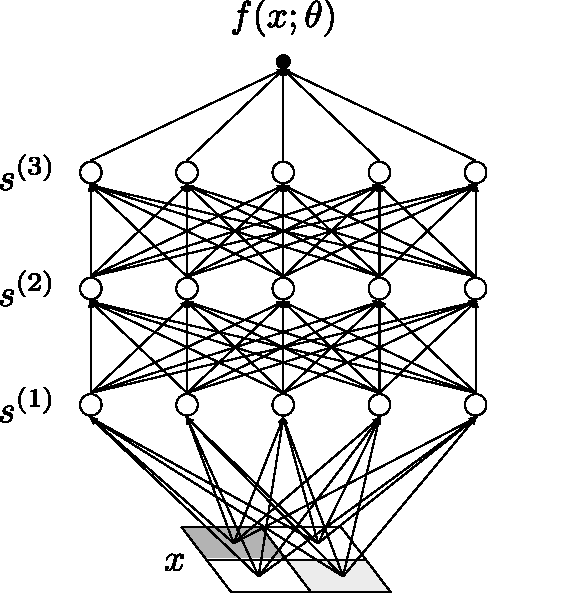
\includegraphics[scale=.7]{./book_figures/mlp-simple.pdf}
\caption{A 
graph
of a simple multilayer neural network, depicting how the input $x$ is transformed through a sequence of intermediate signals, $s^{(1)}$, $s^{(2)}$, and $s^{(3)}$, into the output $f(x;\theta)$.  The white circles represent the neurons, the black dot at the top represents the network output, and the parameters $\theta$ are implicit; they weight the importance of the different arrows carrying the signals and bias the firing threshold of each neuron.
}
\label{fig:mlp-simple}
\end{center}
\end{figure}

For a moment, let's ignore all that structure and simply think of a neural network as a parameterized function
\be
f(x;\theta)\, ,
\ee
where $x$ is the input to the function and $\theta$ is a vector of a large number of \textbf{parameters}\index{model parameters}\index{parameters|see{model parameters}}\index{model parameters|seealso{biases}}\index{model parameters|seealso{weights}} controlling the shape of the function. 
For such a function to be useful,
we need to somehow tune the high-dimensional parameter vector $\theta$.
In practice, this is done in two steps: 
\bi
\item First, we \emph{initialize} the network by randomly sampling the parameter vector $\theta$ from a computationally simple probability distribution,
\be\label{eq:schematic-initialization}
p(\theta)\, .
\ee
We'll later discuss the theoretical reason why it is a good strategy to have an \term{initialization distribution} $p(\theta)$ but, more importantly, this corresponds to what is done in practice, and our approach in this book is to have our theoretical analysis correspond to realistic deep learning scenarios.
\item Second, we adjust the parameter vector as $\theta \to \theta^\star$, such that the resulting \emph{network function} $f(x;\theta^\star)$ is as close as possible to a desired
\emph{target function} $f(x)$: 
\be\label{eq:function-approximation-def}
f(x;\theta^\star) \approx f(x) \, .
\ee
This is called \term{function approximation}\index{function approximation|seealso{machine learning}}.
To find these tunings $\theta^\star$, we 
fit the network function $f(x;\theta)$ to \textbf{training data}\index{training data|see{training set}}\index{training set|textbf}, consisting of many pairs of the form $\big(x, f(x)\big)$ observed from the desired -- but only partially observable -- target function $f(x)$. Overall, making these adjustments to the parameters is called \term{training}\index{training|seealso{gradient descent}}\index{training|seealso{model fitting}}, and the particular procedure used to tune them is called a \textbf{learning algorithm}.\index{learning algorithm}\index{learning algorithm|seealso{Bayesian inference}}\index{learning algorithm|seealso{gradient descent}}
\ei








Our goal is to understand this \emph{trained} network function:
\be\label{eq:lofty-goal}
f(x;\theta^\star)\, .
\ee
In particular, we'd like to understand the macroscopic behavior of this function
from a first-principles microscopic description of the network in terms of these trained parameters $\theta^\star$. We'd also like to understand how the function approximation \eqref{eq:function-approximation-def} works and evaluate how $f(x;\theta^\star)$ uses the training data $\big(x, f(x)\big)$ in its approximation of $f(x)$.
Given the high dimensionality of the parameters $\theta$ and the degree of fine-tuning required for the approximation \eqref{eq:function-approximation-def}, this goal might seem naive and beyond the reach of any realistic theoretical approach. 

One way to more directly see the kinds of technical problems that we'll encounter 
is to \emph{Taylor expand}\index{Taylor series} our trained network function $f(x;\theta^\star)$ around the initialized value of the parameters $\theta$. Being schematic and ignoring for a moment that $\theta$ is a vector and that the derivatives of $f(x;\theta)$ are tensors\index{tensor}, we see
\begin{align}\label{eq:proto-dynamics}
f(x;\theta^\star) =&f(x;\theta) +\dthetaI \frac{df}{d\theta } +\frac{1}{2} \dthetaI^2  \frac{d^2f }{d\theta^2}+\ldots\,,  
\end{align}
where $f(x;\theta)$ and its derivatives on the right-hand side are all evaluated at initialized value of the parameters. This Taylor representation illustrates our three main problems:
\begin{description}
\item[Problem 1]~\\ 
In general, the series \eqref{eq:proto-dynamics} contains an infinite number of terms
\be\label{eq:grand-probelm-1}
f\, ,\quad \frac{df}{d\theta }\, ,\quad \frac{d^2f }{d\theta^2}\, ,\quad \frac{d^3f }{d\theta^3}\,,\quad \frac{d^4f }{d\theta^4}\,,\quad \dots \, , %
\ee
and to use this Taylor representation of the function \eqref{eq:proto-dynamics}, in principle we need to compute them all. 
More specifically, as the difference between the trained and initialized parameters, $\dthetaI$, becomes large, so too does the number of terms 
 needed to get a good approximation of the trained network function $f(x;\theta^\star)$.
\item[Problem 2]~\\ 
Since the parameters $\theta$ are randomly sampled from the initialization distribution, 
$p(\theta)$,
each time we initialize our network 
we get a different function $f(x;\theta)$.
This means that each term $f$, $df/d\theta$, $d^2f/d\theta^2$, \ldots\,, from \eqref{eq:grand-probelm-1} is really a \emph{random function} of the input $x$.
Thus, 
the initialization
induces a distribution over the network function and its derivatives, and we need to determine the mapping,
\be\label{eq:grand-probelm-2}
p(\theta)\to p\!\le(f, \frac{df}{d\theta }, \frac{d^2f }{d\theta^2},\, \dots  \ri) \, ,
\ee
that takes us from the distribution of initial parameters $\theta$ to the \emph{joint} distribution of the network function, $f(x;\theta)$, its \term{gradient}, $df/d\theta$, its \term{Hessian},  $d^2f/d\theta^2$, and so on. This is a joint distribution comprised of an infinite number of random functions,
and in general such functions will have an intricate statistical dependence.
Even if we set aside this infinity of functions for a moment and consider 
just
the
marginal distribution of the network function \emph{only}, $p(f)$, there's still no reason to expect that it's analytically tractable.
\item [Problem 3]~\\
The learned value of the parameters, $\theta^{\star}$, is the result of a complicated training process. In general, $\theta^{\star}$ is not unique and can depend on
\emph{everything}:
\be\label{eq:grand-probelm-3}
\theta^\star \equiv\le[\theta^{\star}\ri]\!\le(\theta,\, f,\, \frac{df}{d\theta},\, \frac{d^2f}{d\theta^2},\, \ldots;\, \text{learning algorithm};\, \text{training data}\ri)\, .
\ee
In practice, the learning algorithm is \emph{iterative}, accumulating changes over many steps, and the dynamics are nonlinear. Thus, the trained parameters $\theta^{\star}$ will depend in a very complicated way on all the quantities at initialization -- such as the specific random sample of the  parameters $\theta$, the network function $f(x;\theta)$ and all of its derivatives, $df/d\theta$, $d^2f/d\theta^2$, \ldots\, -- as well as on the details of the 
learning algorithm and also on the particular pairs, $\big(x, f(x)\big)$, that comprise the training data. Determining an \emph{analytical} expression for $\theta^\star$ must involve taking all of this into account.
\end{description}
If we could solve all three of these problems, then we could in principle use the Taylor-series representation  \eqref{eq:proto-dynamics} to study the trained network function. More specifically, we'd find a \emph{distribution} over trained network functions
\be\label{eq:lofty-goal-refined}
p(f^{\star})\equiv p\Big(f(x;\theta^\star) \Big\vert\, \text{learning algorithm};\, \text{training data} \Big)\, ,
\ee
now conditioned in a simple way on the learning algorithm and the data we used for training. Here, by \emph{simple} we mean that it is easy to evaluate this distribution for different algorithms or choices of training data without having to solve a version of  \textbf{Problem 3} each time. 
The development of a method for the
analytical computation of \eqref{eq:lofty-goal-refined} is a principle goal of this book.

Of course, solving our three problems for a general parameterized function $f(x;\theta)$ is not tractable. However, we are not trying to solve these problems in general; we only care about the functions that are deep neural networks. Necessarily, any solution to the above problems will thus have to make use of the particular \emph{structure} of neural-network function. %
While specifics of how this works form the basis of the book, in the rest of this section we'll try to give intuition for how these complications can be resolved.













\subsubsection{A Principle of Sparsity}
To elaborate on the structure of neural networks, please scroll back a bit and look at Figure~\ref{fig:mlp-simple}.
Note that for the network depicted in this figure, each intermediate or \emph{hidden} layer consists of five neurons, and the input $x$ passes through three such hidden layers before the output is produced at the top after the final layer. In general, two essential aspects of a neural network \neo{architecture} are its \term{width}, $n$, and its \term{depth}, $L$. 











As we foreshadowed in \S\ref{sec:ET-approach}, there are often simplifications to be found in the limit of a large number of components. %
However, it's not enough to consider any massive macroscopic system, and taking the right limit often requires some care.
Regarding the neurons as the components of the network, there are essentially two primal ways that we can make a network grow in size: we can increase its width $n$ holding its depth $L$ fixed, or we can increase its depth $L$ holding its width $n$ fixed.
In this case, it will actually turn out that the former limit will make everything really simple, while the latter limit will be hopelessly complicated and useless in practice.

So let's begin by 
formally taking the limit
\be\label{eq:infinite-width-limit-distribution}
\lim_{n \to \infty} p(f^\star) \, ,
\ee
and studying an \emph{idealized} neural network in this limit.
This is known as the \term{infinite-width limit}\index{infinite-width limit|seealso{not really deep}} of the network, and
as a strict limit
it's rather \emph{unphysical} for a
network: obviously you cannot directly program a function to have an infinite number of components on a finite computer.
However, this extreme limit does massively simplify the distribution over trained networks $p(f^\star)$, rendering each of our three problems completely benign: 
\bi
\item Addressing \textbf{Problem 1}, all the higher derivative terms $d^k f/d\theta^k$ for $k\geq 2$ will effectively vanish, meaning we only need to keep track of two terms,
\be\label{eq:example-of-sparsity-1}
f\, , \quad \frac{df}{d\theta}\, .
\ee
\item Addressing \textbf{Problem 2}, the distributions of these random functions will be independent, 
\be\label{eq:example-of-sparsity-2}
\lim_{n \to \infty}  p\!\le(f, \frac{df}{d\theta}, \frac{d^2f}{d\theta^2},\, \dots  \ri)=p\!\le(f\ri) p\!\le(\frac{df}{d\theta} \ri) \, ,
\ee 
with each marginal distribution factor taking a very simple form. 
\item Addressing \textbf{Problem 3}, the training dynamics become linear and completely independent of the details of the learning algorithm, letting us find a complete analytical solution for $\theta^\star$ in a \emph{closed form}
\be\label{eq:example-of-sparsity-3}
\lim_{n \to \infty}\theta^\star = \le[\theta^{\star}\ri]\!\le(\theta,\, f,\, \frac{df}{d\theta};\, \text{training data}\ri)\, .
\ee
\ei
As a result, the trained distribution \eqref{eq:infinite-width-limit-distribution} is a simple \term{Gaussian distribution} with a nonzero mean, and we can easily analyze the functions that such networks are computing. 










These simplifications are the consequence  of a \textbf{principle of sparsity}\index{sparsity, principle of}.
Even though it seems like we've made the network more complicated 
by growing  it to have an infinite number of components, from the perspective of any particular neuron the 
input of an infinite number of signals is such that the leveling law of large numbers completely obscures much of the details in the signals. The result is that the \emph{effective theory} of many such infinite-width networks leads to extreme sparsity 
in their description,
e.g.~enabling the truncation \eqref{eq:example-of-sparsity-1}. 


Unfortunately, the formal infinite-width limit, $n \to \infty$, leads to a poor model of \emph{deep} neural networks: not only is infinite width an unphysical property for a network to possess, but the resulting trained distribution \eqref{eq:infinite-width-limit-distribution} also leads to a mismatch between theoretical description and practical observation for networks of more than one layer. In particular, it's empirically known that the distribution over such trained networks \emph{does} depend on the properties of the learning algorithm used to train them. Additionally, we will show in detail that such infinite-width networks 
cannot learn representations of their inputs:
for any input $x$, its transformations in the hidden layers, $s^{(1)}$, $s^{(2)}$, \ldots, will remain
unchanged from 
initialization, leading to \emph{random representations}\index{feature function!random}\index{feature function!random|seealso{random feature model}}\index{random feature function|see{feature function}} and thus severely restricting the class of functions that such networks are capable of learning. Since nontrivial \term{representation learning} is an empirically demonstrated essential property of multilayer networks, this really underscores the breakdown of the correspondence between theory and reality in this strict infinite-width limit.

From the theoretical perspective, the problem with this limit is the washing out of the fine details at each neuron due to the consideration of an infinite number of incoming signals. In particular, such an infinite accumulation  completely eliminates the subtle correlations between neurons that get amplified over the course of training for representation learning. To make progress, we'll need to find a way to restore and then study the \term{interactions} between neurons that are present in realistic \emph{finite-width} networks.



With that in mind, perhaps the infinite-width limit can be corrected in a way such that the corrections become small when the width $n$ is large. To do so, we can use \textbf{perturbation theory}\index{perturbation theory} -- just as we do in \terminate{physics} to analyze interacting systems -- and study deep learning using a \textbf{1/\emph{n} expansion}\index{$1/n$ expansion|textbf}, treating the inverse layer width, $\epsilon \equiv 1/n$, as our small parameter of expansion: $\epsilon \ll 1$. 
In other words, we're going to back off the strict infinite-width limit and compute the trained distribution \eqref{eq:lofty-goal-refined} with the following expansion:
\be\label{eq:finite-width-limit-distribution}
p(f^\star) \equiv p^{\{0\}}(f^\star) + \frac{p^{\{1\}}(f^\star) }{n} + \frac{p^{\{2\}}(f^\star) }{n^2} + \dots \, ,
\ee
where $p^{\{0\}}(f^\star) \equiv \lim_{n\to \infty} p (f^\star)$ is the infinite-width limit we discussed above, \eqref{eq:infinite-width-limit-distribution}, and the $p^{\{k\}}(f^\star)$ for $k \geq 1 $ give a series of corrections to this limit. 

In this book, we'll in particular compute the first such correction, truncating the expansion as
\be\label{eq:finite-width-limit-distribution-truncated}
p(f^\star) \equiv p^{\{0\}}(f^\star) + \frac{p^{\{1\}}(f^\star) }{n} + \o{\frac{1}{n^2}} \, .
\ee
This \neo{interacting theory} is still simple enough to make our three problems tractable: 
\bi
\item Addressing \textbf{Problem~1}, now all the higher derivative terms $d^k f/d\theta^k$ for $k\geq 4$ will effectively give contributions  of the order $1/n^2$ or smaller, meaning that to capture the leading contributions of order $1/n$, we only need to keep track of four terms:
\be\label{eq:example-of-sparsity-finite-n-1}
f\, , \quad \frac{df}{d\theta}\, , \quad \frac{d^2f}{d\theta^2}\,, \quad \frac{d^3f}{d\theta^3}\, .
\ee
Thus, we see that the \emph{principle of sparsity}\index{sparsity, principle of} will still limit the dual\index{duality} effective theory description, though not quite as
extensively
as in the infinite-width limit.
\item Addressing \textbf{Problem~2}, the distribution of these random functions at initialization,
\be\label{eq:example-of-sparsity-finite-n-2}
p\!\le(f, \frac{df}{d\theta }, \frac{d^2f}{d\theta^2 },\frac{d^3f}{d\theta^3}  \ri)\, ,
\ee
will be \emph{nearly} simple at order $1/n$, and we'll be able to work it out in full detail using perturbation theory. 
\item Addressing \textbf{Problem~3}, we'll be able to use a dynamical perturbation theory to tame the nonlinear training  dynamics and find an analytic solution for $\theta^\star$ in a \emph{closed form}:
\be\label{eq:example-of-sparsity-finite-n-3}
\theta^\star=\le[\theta^{\star}\ri]\le(\theta, f,\, \frac{df}{d\theta}\, ,\frac{d^2f}{d\theta^2}\, \frac{d^3f}{d\theta^3};\, \text{learning algorithm};\, \text{training data}\ri)\, .
\ee
In particular, this will make the dependence of the solution on the details of the learning algorithm transparent and manifest.
\ei
As a result, our description of the trained distribution at order $1/n$, \eqref{eq:finite-width-limit-distribution-truncated},  will be a \term{nearly-Gaussian distribution}. 





In addition to being analytically tractable, this truncated description at order $1/n$ will satisfy our goal of computing and understanding the distribution over trained network functions
$p(f^\star)$. As a consequence of incorporating the interactions between neurons, this description has a dependence on the details of the learning algorithm and, as we'll see, includes nontrivial representation learning. Thus, \emph{qualitatively}, this effective theory at order $1/n$ corresponds much more closely to realistic neural networks than the infinite-width description, making it far more useful as a theoretically \term{minimal model} for understanding deep learning. 

How about the quantitative correspondence? As there is a sequence of finer descriptions that we can get by computing higher-order terms in the expansion \eqref{eq:finite-width-limit-distribution}, do these terms also need to be included?
 
While the formalism we introduce in the book makes computing these additional terms in the \terminate{$1/n$ expansion} completely systematic -- though perhaps somewhat tedious -- an important byproduct of studying the leading correction is actually a deeper understanding of this truncation error. In particular, what we'll find is that the correct scale to compare with width $n$ is the depth $L$. That is, we'll see that the relative magnitudes of the terms in the expansion \eqref{eq:finite-width-limit-distribution} are given by the depth-to-width aspect ratio: 
\be
r \equiv L/n\, .
\ee
This lets us recast our understanding of infinite-width vs.~finite-width and shallow vs.~deep in the following way:
\bi
\item In the strict limit $r \to 0$, the interactions between neurons turn off: the infinite-width limit \eqref{eq:infinite-width-limit-distribution} is actually a decent description. However, these networks are \neo{not really deep}\index{not really deep|seealso{infinite-width limit}}, as their relative depth is zero: $L/n =0$. 
\item
In the regime $0 < r \ll 1$, there are nontrivial interactions between neurons: the finite-width effective theory truncated at order $1/n$, \eqref{eq:finite-width-limit-distribution-truncated}, gives an accurate accounting of the trained network output.
These networks are \neo{effectively deep}.\index{effectively deep|seealso{optimal aspect ratio}}
\item In the regime $ r \gg 1$, the neurons are strongly coupled: networks will behave chaotically,
and there is no effective description due to large fluctuations from instantiation to instantiation. These networks are \neo{overly deep}.\index{overly deep|seealso{degradation problem}}\index{overly deep|seealso{chaos}}
\ei 
As such, most networks of practical use actually have reasonably small depth-to-width ratios, 
and so our
truncated description at order $1/n$, \eqref{eq:finite-width-limit-distribution-truncated}, will provide a great \emph{quantitative} correspondence as well.\footnote{More precisely, there is an \neo{optimal aspect ratio}\index{optimal aspect ratio|seealso{effectively deep}}, $r^{\star}$, that divides the effective regime $r \leq r^{\star}$ and the ineffective regime $r > r^{\star}$. In Appendix~\ref{app:mi-stuff}, we'll estimate this \terminate{optimal aspect ratio} from an information-theoretic\index{information theory}\index{information theory|seealso{statistical mechanics}} perspective. In Appendix \ref{app:residual}, we'll further show how \emph{residual connections}\index{residual connection} can be introduced to shift the optimal aspect ratio $r^{\star}$ to larger values, making the formerly overly-deep networks 
more practically trainable as well as quantitatively describable by our 
effective theory approach.}

From this, we see that to really describe the properties of \emph{multilayer} neural networks, i.e.~to understand \neo{deep learning}, we need to study large-but-finite-width networks. In this way, we'll be able to find a macroscopic \emph{effective theory} description of realistic deep neural networks.




























 


























